\chapter{آموزش ورژن کنترل}




\section{مقدمه}
ورژن کنترل چیست ؟ و چرا باید به آن اهمیت دهیم ؟ ورژن کنترل یک سیستم ذخیره سازی یک یا چند فایل در طول زمان است \cite{Blischak2016} ورژن کنترل سیستمی است که به توسعه‌دهندگان نرم‌افزار کمک می‌کند تا علاوه بر امکان مشارکت روی پروژه‌های نرم‌افزاری، بتوانند به تاریخچه‌ای از کدهایی که قبلاً نوشته‌اند نیز دست پیدا کنند و به طور کلی اهداف استفاده از سیستم‌های ورژن کنترل را می‌توان در موارد زیر خلاصه نمود:
- فراهم آوردن فرصتی برای توسعه‌دهندگان به منظور کار کردن به صورت هم‌زمان 
- مجزاسازی نسخه‌های توسعه داده شده اختصاصی تک‌تک توسعه‌دهندگان 
- نگهداری تاریخچه‌ای از هر نسخه از هر چیزی که به اشتراک گذاشته شود.
با استفاده از ورژن کنترل شما می توانید ایده های جدید خود را بدون نگرانی آزمایش کنید و در صورت نیاز به ورژن های قبلی برگردید\cite{Chacon2014}. ورژن کنترل سیستمی ضروری برای کار گروهی بر روی یک پروژه نرم افزاری است \cite{DeAlwis2009} . 
گیت یک نرم‌افزار کنترل نسخه و از مدل نرم‌افزارهای متن‌باز برای بازنگری کدمنبع توزیع شده و مدیریت منبع کد است که برای دنبال کردن تغییر فایلهای کامپیوتری و دنبال کردن کارهای انجام شده روی آن‌ها توسط افراد مختلف است. که در تمامی سیستم عامل های اصلی توسعه داده شده است \cite{Ram2013} . گیت یک راه قدرتمند برای ردیابی و مقایسه نسخه ها، رفع خطاها، کشف رویکردهای جدید به شیوه ای ساختاری است\cite{spinellis2012git} .
گیت ابتدا برای توسعه لینوکس توسط لینوس تُروالدز به وجود آمد و اکنون پروژه‌های فراوانی از آن الهام گرفته‌اند. هر دایرکتوری کاری در گیت یک مخزن کامل با تاریخچه کامل تغییرها و قابلیت بازنگری آن‌ها است و برای کار با آن نیازی به دسترسی به شبکه یا سرور مرکزی وجود ندارد.
امروزه برنامه نویسی که به گیت مسلط نباشد را عملا برنامه نویس نمیدادند، به عبارت دیگر تسلط به گیت وظیفه ی هر برنامه نویس میباشد. در هرپروژه ای در هر سطحی در دنیا و در هر شرکتی از گیت استفاده میشود حتی شرکت های غیر برنامه نویسی مانند مقاله نویسی ، پایان نامه و هر نوع فایل متنی دیگری میتوان از گیت استفاده نمود؛ مانند همین مقاله که با استفاده از گیت انجام شده است! پس با ما در ادامه این آموزش همراه باشید چون با همین اطلاعات و تمرین آن ها میتوانید آشنایی با گیت را در رزومه خود اضافه کنید.

\newpage

\section{تاریخچه}
اینجا ی چیزایی راجبه تاریخش بنویس و سع یکن رفرنس بدی بجز اینجا جای دیگ رفرنس نداریم 
\section{کنترل منابع \lr{(Source control)}}
ی چیز در مورد سرس کنترل بنویس بازار و cvn و ..... اینا رو هم بگو 



\section{گیت \lr{(Git)}}
در این پژوهش به کارایی گیت و همچنین نحوه اجرای دستورات مختلف آن آشنا خواهید شد.
\subsection{شروع کار با گیت}
برای شروع کار با گیت باید نرم افزار گیت را در سیستم خود نصب نمایید.
سپس با با ساختن یک \lr{git dash} در مسیری که میخواهید پروژه خود را شروع کنید صفحه ای باز میشود و میتوانیم در آن دستورات گیت را اجرا کنیم. برای شروع نیاز به دانستن دو نوع شروع پروژه یا ساخت مخزن داریم:
\begin{figure}[tbh]
	\centering
	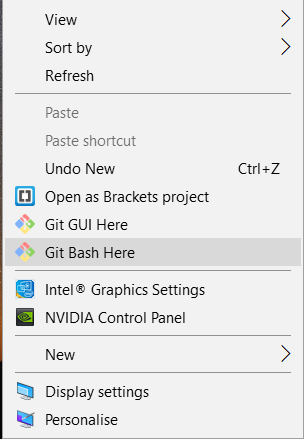
\includegraphics{./Figures/GitBash}
	\caption{ چگونگی ساختن گیت bash  }
	\label{Fig:GitBash}
\end{figure}
\subsubsection{init}
دستور \lr{git init} یک مخزن (repository) جدید ایجاد میکند. این دستور برای تبدیل یک پروژه موجود که ورژنش مشخص نشده به یک مخزن گیت یا ساختن   مخزن جدید خالی مورداستفاده قرار میگیرد. \newline
بقیه دستورات گیت خارج از محدوده ی یک مخزن گیت ساخته شده نیستند. پس بطور معمول این دستور اولین دستور است که شما آن را در یک پروژه جدید اجرا میکنید. \newline
اجرای دستور \lr{git init} یک زیرشاخه دستور \lr{.git } در شاخه ی جاری در حال استفاده میسازد که شامل تمامی متادیتاهایی است که گیت برای ساختن یم مخزن جدید به آن ها نیاز دارد. این متادیتا شامل زیرشاخه ها،مراجع , قالب فایل هااست. \newline
درکنار شاخه \lr{.git } در شاخه ریشه پروژه ، یک پروژه موجود باقی می ماند بدون تغییر میماند.  \newline
به طور پیش فرض، دستور init پیکربندی Git را به مسیر زیرشاخه .git راه اندازی خواهد کرد. مسیر دلخواه را می توانید تغییر دهید و سفارشی کنید اگر دوست دارید آن را در جای دیگر اسفاده کنید. شما می توانید متغیر محدوده  \lr{GIT-DIR } را به یک مسیر سفارشی تنظیم کنید و در ابتدا دستور init فایل های پیکربندی Git را در آنجا راه اندازی خواهد کرد. علاوه بر این شما می توانید یک آرگومان separate-git-dir برای نتیجه ی مشابه منتقل کنید. یک مورد استفاده معمول برای یک زیرگروه جداگانه .git این است که پیکربندی سیستم شما را در پوشه اصلی حفظ کند و پوشه .git را در جای دیگر نگه دارد.
\newline
\begin{figure}[tbh]
	\centering
	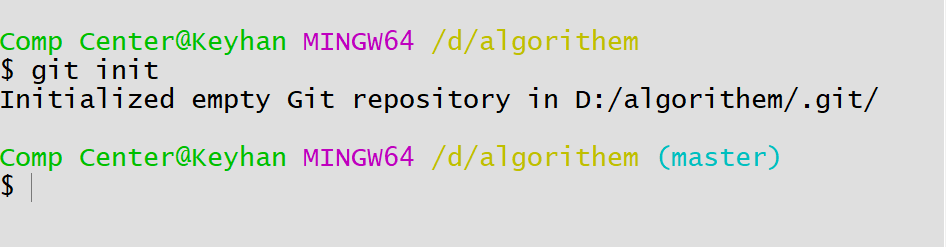
\includegraphics[width=1\textwidth]{./Figures/GitInit}
	\caption{ اعمال دستور init بر روی یک شاخه دلخواه در محیط گیت bash }
	\label{Fig:GitInit}
\end{figure}

\newpage
\subsubsection{clone}
این دستور برای دانلود یک ریپازیتوری موجود در شبکه استفاده میشود. در واقع ما میتوانیم با استفاده از این دستور یک فایل .git موجود در شبکه که میتواند سایت هایی مانند gitlab یا github و یا گیت شرکت شما باشد را در یکی از شاخه های سیستم خودمان داشته باشیم. مانندشکل \ref{Fig:GitClone}    \newline این دستور عینا پروژه را در مسیر منتخب شما کپی میکند، و شما میتوانید آن را تغییر داده و ادامه دهید. \newline گیت کلون تنها یک کپی کاری ساده نیست، بلکه با این دستور شما در واقع یک کپی از تمامی اطلاعاتی که سرور دارد است. تمامی ورژن ها ، تغییرات اعمال شده بر آنها در طول زمان است. \newline در حقیقت، اگر دیسک سرور شما خراب شود، شما اغلب می توانید تقریبا هر یک از کلون ها را بر روی هر سیستمی در شبکه بکار ببندید تا سرور را به حالت ای که در زمان کپی شدن آن بود، بازگردانید.  
\newline
\newline
\begin{figure}[tbh]
	\centering
	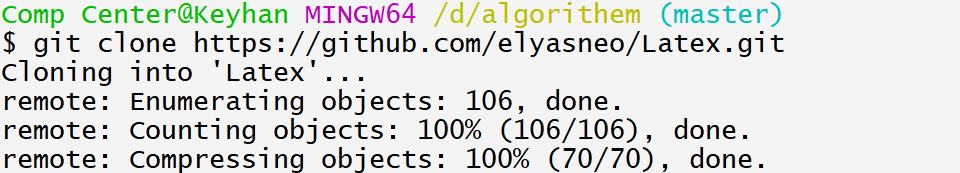
\includegraphics[width=1\textwidth]{./Figures/GitClone}
	\caption{ دانلود روند همین پروژه از گیت لب از پروژه مشترکان   }
	\label{Fig:GitClone}
\end{figure}
\subsection{بررسی و دستیابی}
یکی از محاسن گیت این است که ما میتوانیم در هر لحظه تغیررات ایجاد شده بر روی هر فایل را مشاهده کنیم ! فایل های تغییر یافته را بشناسیم و در کل وضعیتی که داریم را مشاهده کنیم. همینطور میتوانیم به گذشته برویم و به ورژن های مختلف دسترسی داشته باشیم.
این ویژگی بسیار در کار ما با گیت اهمیت دارد زیرا گاها پیش می آید که فرضا در حین انجام یک بخش از کار نیاز به نصب نرم افزار بر یک سیستم یا ایجاد یک باگ شود که نیاز به دسترسی به نسخه های قبلی برای نصب و یا ایراد یابی باشد. 
\subsubsection{status}
دستور گیت status  وضعیت دایرکتوری کار و منطقه پیمایش را نمایش می دهد. این به شما اجازه می دهد ببینید کدام تغییرات مرتب شده اند و کدام فایل ها توسط Git ردیابی نمی شوند. خروجی این دستور شما هیچ اطلاعاتی را نشان نمی دهد برای این کار باید از گیت log استفاده کنید. شکل های را ببینید: \ref{Fig:GitStatus} در این تصویر فایل های قرمز ابتدایی فایل های تغییر یافته و فایل های قسمت دوم فایل های که توسط گیت ردیابی نمیشوند را نمایش میدهد.  
\begin{figure}[tbh]
	\centering
	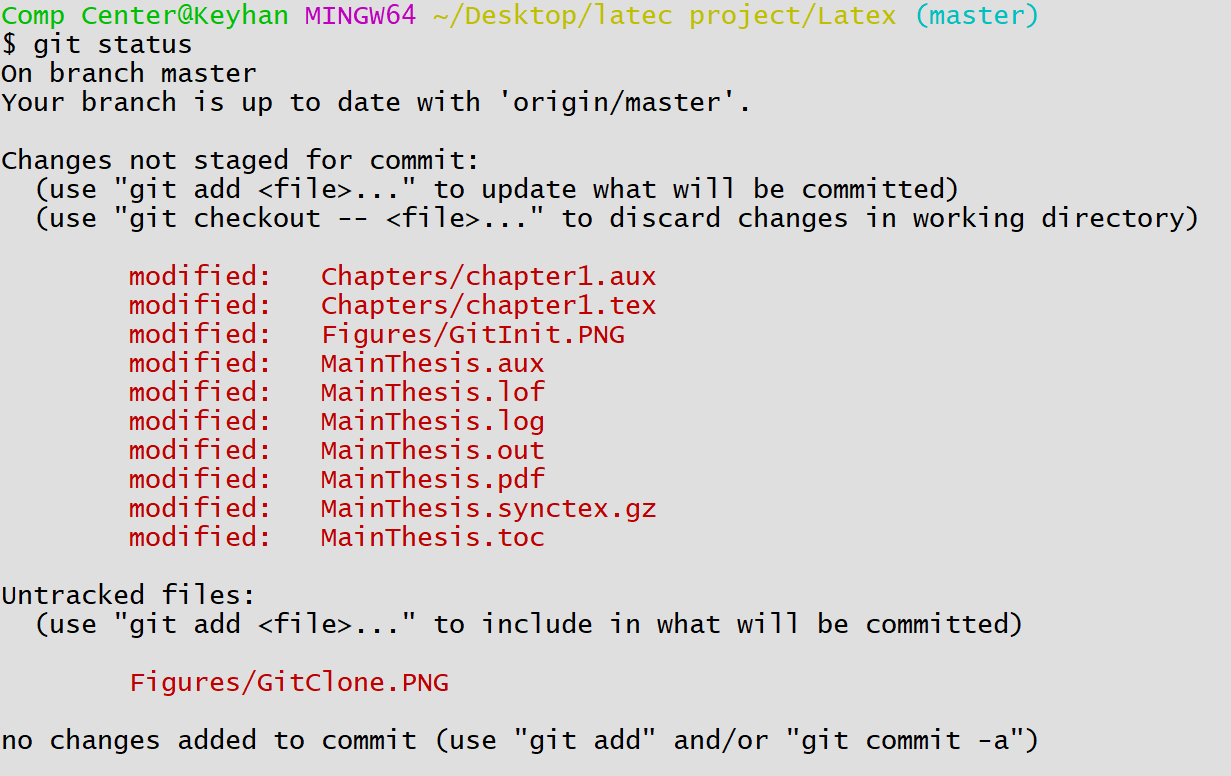
\includegraphics[width=1\textwidth]{./Figures/GitStatus}
	\caption{ گیت استتوس بر روی روند مقاله فعلی بر شاخه .git }
	\label{Fig:GitStatus}
\end{figure}
\newpage
\subsubsection{log}
با اجرای این دستور لیستی از کامیت هایی که تاکنون بر روی شاخه انجام شده است مشاهده میشود، شکل را ببینید: \ref{Fig:GitLog}
\begin{figure}[tbh]
	\centering
	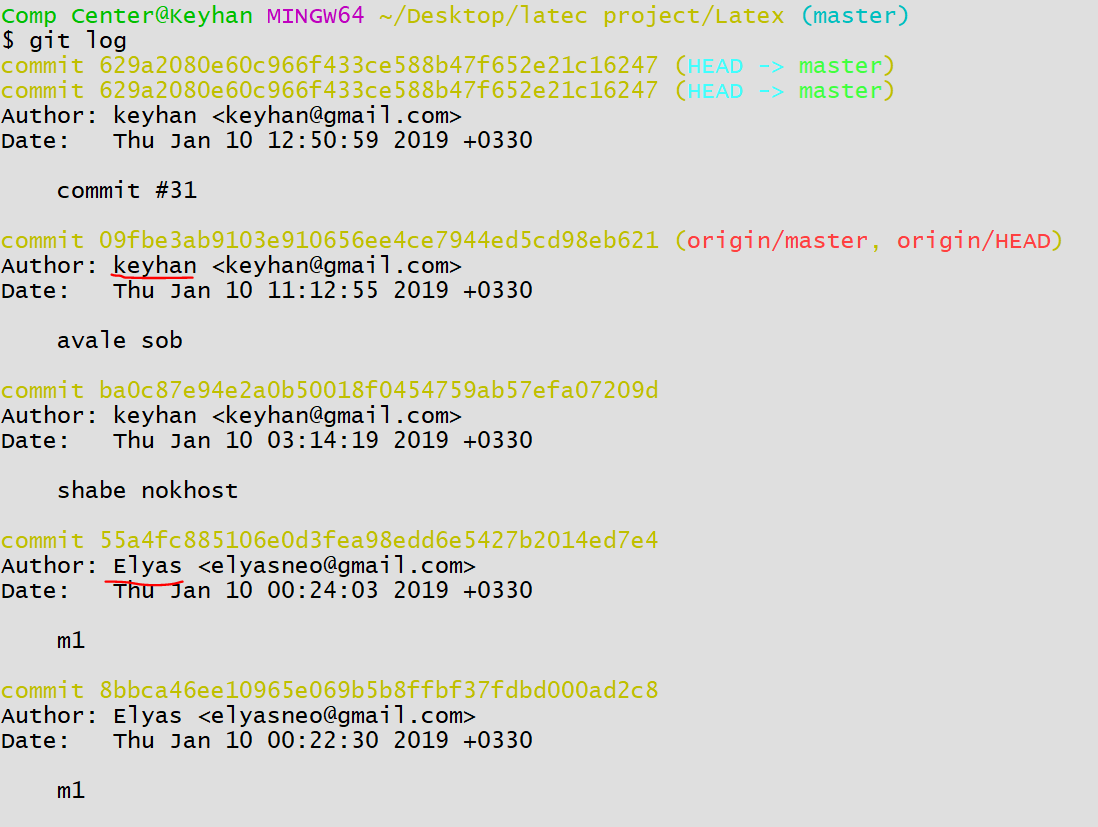
\includegraphics[width=1\textwidth]{./Figures/GitLog}
	\caption{ کامیت های انجام شده بر روی مقاله کنونی تا بدینجای کار }
	\label{Fig:GitLog}
\end{figure}
\subsubsection{diff}
\subsubsection{checkout}
دستور checkout عمل تغییر بین نسخه های مختلف یک موجودیت هدف است. این دستور بر روی سه موجودیت مجزا عمل می کند: فایل ها، commit ها، و شاخه ها. علاوه بر تعریف «checkout»، عبارت «چک کردن» معمولا به معنای اجرای دستور فرمان گیت checkout است. در موضوع لغو تغییرات، ما شاهد چگونگی استفاده از گیت  Checkout برای مشاهده اعمال قدیمی بودیم. اکثر تمرکزاین سند بر عملیات checkout در شاخه ها است.
\newline
چک کردن شاخه ها مشابه چک کردن قرارداد های قدیمی و فایل ها در آن است که دایرکتوری کاری برای مطابقت با شاخه انتخاب شده به روز می شود؛ با این حال، تغییرات جدید در تاریخ پروژه ذخیره می شود - یعنی یک عملیات فقط خواندنی نیست. \newline
در شکل \ref{Fig:GitCheckout} ابتدا به یک نسخه قدیمی میرویم و بعد در شکل \ref{Fig:GitCheckout2} با دستور بعدی به ورژن فعلی برمیگردیم!
\newline
\begin{figure}[tbh]
	\centering
	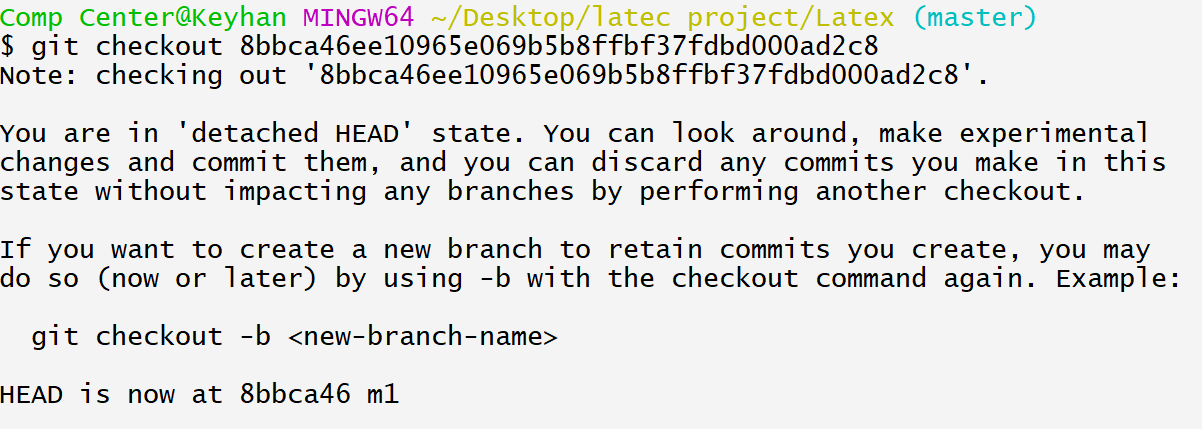
\includegraphics[width=1\textwidth]{./Figures/GitCheckout}
	\caption{ به ورژن های قبلی}
	\label{Fig:GitCheckout}
\end{figure}
\begin{figure}[tbh]
	\centering
	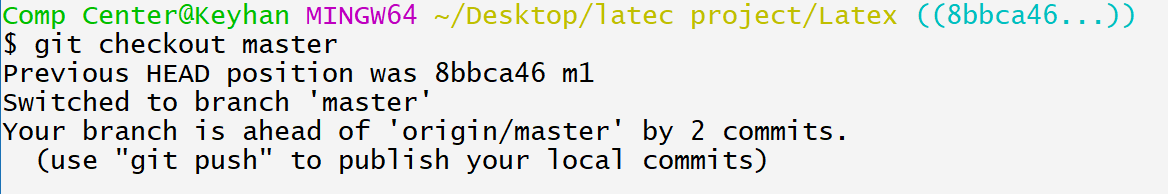
\includegraphics[width=1\textwidth]{./Figures/GitCheckout2}
	\caption{ برگشت به ورژن master }
	\label{Fig:GitCheckout2}
\end{figure}
